% ---------------------------------------------------------------------------- %
\subsection{Produktumfeld}
% ---------------------------------------------------------------------------- %


Das   Projekt   kann  grob   in   vier   Teilgebiete  unterteilt   werden: Die
Spannungsmessung, die Daten\"ubertragung, die Datenauswertung und die Speisung
des Sensors bzw. der Zentrale.


% ---------------------------------------------------------------------------- %
\subsection{Produkteigenschaften}
\label{subsec:produkteigenschaften}
% ---------------------------------------------------------------------------- %

Unser  Produkt  dient  zur  \"Uberwachung der  Spannung  an  Solarmodulen. Die
gemessene Spannung  pro Modul wird  \"uber die  DC Leitung der  Solaranlage zu
einem Masterger\"at \"ubertragen, welcher die gemessenen Werte verarbeitet und
allf\"allige  Fehler erkennt. Tritt  ein Fehler  auf, wird  eine entsprechende
Meldung  auf einem  Display  angezeigt, ein  Relais  f\"ur eine  zus\"atzliche
Alarmierung bet\"atigt und eine  Nachricht mittels SMS versendet. Dadurch wird
sichergestellt, dass defekte Solarmodule m\"oglichst schnell erkannt werden.

Die Bedienung des  Produktes wird einfach gehalten. Mittels  Touch Display auf
dem Masterger\"at k\"onnen die  n\"otigen Grundeinstellungen get\"atigt werden
und im  Fehlerfall wird die  Bezeichung des fehlerhaften  Moduls angezeigt. Im
Normalbetrieb muss keine Bedienung erfolgen.

Installiert  wird  der  Master beim  Generatoranschlusskasten  (GAK). Er  wird
in  Form  eines  Hutschienenger\"at  (REG)  produziert,  zur  Montage  in  das
bestehend GAK. Damit wird ein kleinst m\"oglicher Montagaufwand erreicht.  Die
Sensorplatine wird  bei jedem Modul in  der Modulanschlussbox installiert. Aus
diesem Grund wird der Sensor m\"oglichst klein, jedoch nicht wasserfest.

\textsc{TODO}: Genaue Definition eines Fehlers (Feedback)


% ---------------------------------------------------------------------------- %
\subsection{Systembereich}
% ---------------------------------------------------------------------------- %

Das      System      (schematische       Darstellung      siehe      Abbildung
\ref{fig:blockdiag:hardware})     besteht     grunds\"atzlich     auf     zwei
Teilsysteme. Einerseits aus der Sensorplatine, welche in der Modulanschlussbox
platziert   ist,   andererseits   aus    dem   Masterger\"at,   welches   beim
Generatoranschlusskasten installiert ist.

Die Sensorplatine ist nur f\"ur die Datenerfassung zust\"andig.

%\textsc{TODO}: Noch ein wenig ausformulieren.
\begin{figure}[h!]
    \centering
    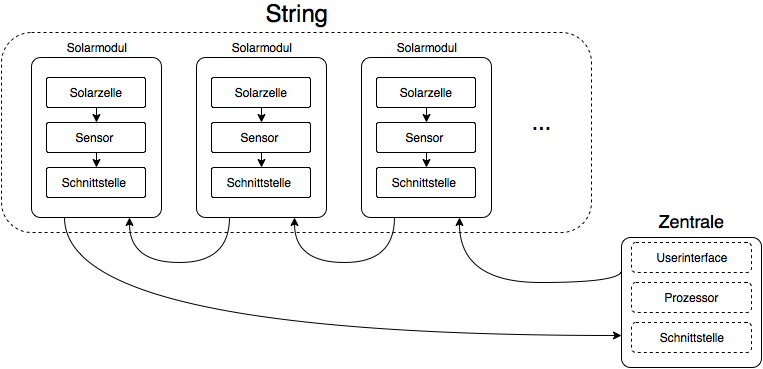
\includegraphics[width=.9\textwidth]{images/blockdiag.png}
    \caption{Blockdiagramm Hardwareaufbau}
    \label{fig:blockdiag:hardware}
\end{figure}


% TODO
% ---------------------------------------------------------------------------- %
\subsection{L\"osungsvarianten}
\label{subsec:losungsvarianten}
% ---------------------------------------------------------------------------- %

Es   wurden  drei   Methoden  evaluiert,   um  ein   Signal  ohne   dedizierte
Datenleitungen zu \"ubertragen.

Eine erste Methode ist die Verwendung eines fertig entwickelten Chips.  Solche
Chips sind  praxiserprobt und  garantieren Funktionalit\"at.  Jedoch  sind sie
\"uberladen mit Features und verh\"altnism\"assig teuer.

Alternativ  kann  mittels  eines   PLL-Chips  FSK  moduliert  und  demoduliert
werden. Fertige Chips basieren  ebenfalls auf diesem Prinzip,  jedoch ist eine
L\"osung mit  PLL-Chip und Peripherie  wesentlich g\"unstiger (Faktor  10) als
eine auf einem fertigen Chip basierende L\"osung.

Diese  beiden   Methoden  m\"ussten   induktiv  oder   kapazitiv  eingekoppelt
werden. Induktiv   ist  potentialgetrennt   und  braucht   wesentlich  weniger
Energie. Kapazitiv ist daf\"ur in der  Herstellung viel g\"unstiger und in der
Baugr\"osse wesentlich kleiner.

Eine letzte  m\"ogliche Methode besteht  darin, mit einem Mosfet  die Spannung
\"uber der  Solarzelle mit einem Kurzschluss  einbrechen zu lassen und  so die
einzelnen  Bits amplitudenmoduliert  zu  \"ubertragen. Diese  Methode ist  die
kompakteste und  ist ein wenig kostspieliger  als die zweite aber  dennoch bei
weitem g\"unstiger  als die  erste. Ein Wermutstropfen  ist dabei,  dass diese
Daten\"ubertragung  lediglich  unidirektional  realisierbar  w\"are,  da  beim
Masterger\"at die  Spannung bzw. der Strom  zu hoch ist, um  dort die Spannung
einbrechen zu lassen.

Die  kostspieligste Variante  wurde f\"urs  erste ausgeschlossen. Die  anderen
zwei werden intensiv getestet.

Eine    \"Ubersicht     der    Vor-    und    Nachteile     liefert    Tabelle
\ref{tab:signalvariants}.

\begin{table}[h!]
    \centering
    \small
    \caption{Variantenvergleich f\"ur Signal\"ubertragung}
    \label{tab:signalvariants}
    \begin{tabular}{
        >{\raggedright}p{6mm}|
        >{\raggedright}p{40mm}
        >{\raggedright}p{40mm}
        >{\raggedright\arraybackslash}p{40mm}}

        \toprule
        & \textsc{Fertiger Chip}
        & \textsc{Eigene FSK}
        & \textsc{Short-Circuit}
        \\
        \midrule
        & funktioniert mit grosser Wahrscheinlichkeit
        & kosteng\"unstig
        & kosteng\"unstig
        \\

        \rowcolor{black!10}
        \cellcolor{white}
        & zertifiziert
        & bekanntest System
        & sehr einfacher Schaltungsaufbau
        \\

        & geringerer Entwicklungsaufwand
        & einfache Fehlersuche
        & geringerer Entwicklungsaufwand
        \\


        \rowcolor{black!10}
        \parbox[t]{1em}{\cellcolor{white}\multirow{-4}{*}{\rotatebox[origin=c]{90}{pro}}}
        &
        & bew\"ahrtes Grundprinzip
        &
        \\

        \midrule
        & sehr teuer
        & h\"ohrerer Entwicklungsaufwand
        & ungetestes Prinzip
        \\

        \rowcolor{black!10}
        \cellcolor{white}
        & unbekanntes System (Black Box)
        & fehleranf\"alliger, weniger robust
        & hitzeentwicklung beim Schalten allenfalls problematisch
        \\

        & erschwerte Fehlersuche (System komplexer)
        & potentiell h\"oherer Stromverbrauch
        & Signal wird nicht durch das IC getrieben
        \\


        \rowcolor{black!10}
        \parbox[t]{1em}{\cellcolor{white}\multirow{-4}{*}{\rotatebox[origin=c]{90}{contra}}}
        & viele nicht ben\"otigte Funktionen (komplexeres System, h\"ohere Kosten)
        &
        &
        \\

        \bottomrule
    \end{tabular}
\end{table}

\textsc{TODO}: varianten RasPi vs. Alternativen?

% TODO
% ---------------------------------------------------------------------------- %
%\subsection{Evaluation L\"osungsvarianten}
% ---------------------------------------------------------------------------- %
%\textsc{TODO}
